\subsection{Łatwiejsze enumerowanie z {\tt yield}}

W podrozdziale~\ref{IEnumerable} mieliśmy możliwość zobaczyć w jaki sposób za pomocą pary interfejsów 
{\tt IEnumerable} i {\tt IEnumerator} można zdefiniować obiekty o enumerowalnej zawartości. Szczególne wygodna
jest możliwość stosowania lukru syntaktycznego {\tt foreach (...)} dzięki której kod enumerowania jest zwięzły i 
jednorodny (niezależny od szczegółów wewnętrznej implementacji enumerowanej klasy).

Największą słabością tego podejścia jest jej uciążliwość, jest to szczególnie widoczne wtedy kiedy enumerowany obiekt
nie ma prostej, liniowej struktury. Rozważmy przykład drzewa binarnego z rysunku~\ref{fig:pbintree}.

\begin{figure}
\begin{center}
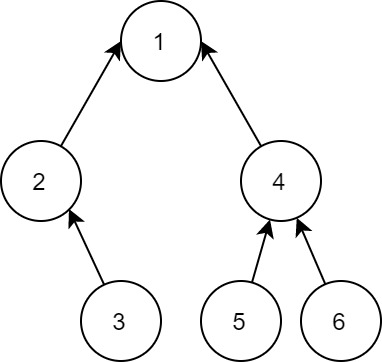
\includegraphics[width=0.50\textwidth]{./pic/tree}
\caption{Proste drzewo binarne}
\label{fig:pbintree}
\end{center}
\end{figure}

Implementacja struktury mogłaby wyglądać tak:

\begin{scriptsize}
\begin{verbatim}
public class Tree
{
    public Tree Left { get; set; }
    public Tree Right { get; set; }
    public int Value { get; set; }
}

class Program
{
    static void Main(string[] args)
    {
        Tree root  = new Tree();
        root.Value = 1;

        Tree left  = new Tree();
        left.Value = 2;

        Tree subleft  = new Tree();
        subleft.Value = 3;
        left.Right    = subleft;

        Tree right = new Tree();
        right.Value = 4;

        Tree subright1  = new Tree();
        subright1.Value = 5;
        right.Left      = subright1;
        Tree subright2  = new Tree();
        subright2.Value = 6;
        right.Right     = subright2;

        root.Left  = left;
        root.Right = right;
    }
}
\end{verbatim}
\end{scriptsize}

To bardzo dobra struktura danych do napisania 

\begin{scriptsize}
\begin{verbatim}
foreach ( var elem in root ) 
{

}

// zwraca 1, 2, 3, 4, 5, 6
\end{verbatim}
\end{scriptsize}

ale oczywiście brakuje tu enumeratora. 

Jego implementacja według specyfikacji {\tt IEnumerable} jest zaskakująco nieoczywista. Problem polega na tym 
że wywołanie metody {\tt MoveNext}, które przesuwa enumerator na "kolejny element" tu musi przesuwać go po strukturze
rekurencyjnej w taki sprytny sposób, żeby odwiedzając węzeł jakoś (jak?) wiedzieć, czy to jest to wywołanie w którym
enumerator przesunie się "w głąb" struktury, do węzłów-dzieci, czy też może węzły-dzieci już zostały odwiedzone więc
należy wrócić do węzła-ojca i szukać innej scieżki, do kolejnych, sąsiednich gałęzi.

Poprawny sposób odwiedzania węzłów drzewa binarnego wynika dopiero z wiedzy o strukturach danych. W tym przypadku
algorytm wykorzysta dodatkową, pomocniczą strukturę danych do zapamiętania odwiedzonych węzłów. Tą dodatkową pomocniczą
sturkturą danych będzie albo stos - dla algorytmu odwiedzania drzewa wgłąb albo kolejka - dla algorytmu odwiedzania 
odwiedzania drzewa wszerz.

Okazuje się, że metoda {\tt MoveNext} implementowana przy pomocy dodatkowej, 
pomocniczej struktury danych, może być całkiem prosta:

\begin{enumerate}
\item do pomocniczej struktury włoż korzeń drzewa
\item powtarzaj
    \begin{enumerate}
    \item wyjmij element z pomocniczej struktury, zapamiętaj go jako wartość zwracaną z {\tt Current}
    \item do pomocniczej struktury włóż dzieci zdjętego węzła (jeśli istnieją)
    \item jeśli struktura jest niepusta zwróć {\tt true}, w przeciwnym razie zwróć {\tt false}
    \end{enumerate}
\end{enumerate}

Czytelnikowi jako ćwiczenie pozostawia się sprawdzenie że ten prosty algorytm zachowuje się faktycznie podobnie
dla struktury stosu i kolejki, w obu tych przypadkach zapewniając inną strategię odwiedzania węzłów drzewa.

Kod w języku C\# odpowiadający temu algorytmowi dla struktury drzewa wyglądać mógłby tak:

\begin{scriptsize}
\begin{verbatim}
public class Tree : IEnumerable
{
    public class TreeEnumerator : IEnumerator
    {
        private Stack stack = new Stack();

        private Tree root; // zawsze korzeń
        private Tree curr; // bieżący element

        public TreeEnumerator( Tree tree )
        {
            this.root = tree;

            this.Reset();
        }

        public object Current
        {
            get
            {
                if (curr != null)
                {
                    return curr.Value;
                }
                else
                {
                    throw new ArgumentException("Brak elementu do zwrócenia wartości");
                }
            }
        }

        public bool MoveNext()
        {
            if ( stack.Count > 0 )
            {
                // zdejmij element ze stosu
                curr = (Tree)stack.Pop();

                // do stosu dodaj jego poddrzewo
                if (curr.Right != null) stack.Push(curr.Right);
                if (curr.Left != null) stack.Push(curr.Left);

                // enumeruj dalej
                return true;
            }
            else
            {
                return false;
            }
        }

        public void Reset()
        {
            stack.Clear();
            stack.Push(this.root);
            this.curr = this.root;
        }
    }

    public Tree Left { get; set; }
    public Tree Right { get; set; }
    public int Value { get; set; }

    public IEnumerator GetEnumerator()
    {
        return new TreeEnumerator(this);
    }
}
\end{verbatim}
\end{scriptsize}

Czytelnik jest proszony o sprawdzenie że taka implementacja istotnie pozwala enumerować zawartość
drzewa wgłąb za pomocą {\tt foreach} i że zamiana stosu na kolejkę (oraz jeszcze jeden szczegół) pozwala
enumerować zawartość wszerz.

To co warto zauważyć, to to że bez pomocniczej struktury implementacja mogłaby być jeszcze bardziej
skomplikowana (jak bardzo?) ale nawet to nie pomaga poradzić sobie z technicznymi uciążliwościami wynikającymi
z rozdzielenia implementacji {\tt MoveNext} i {\tt Current}, która wymusza zapamiętywanie "bieżącego elementu"
po to żeby można go było zwrócić.

Okazuje się, że implementacja enumeratora może być znacznie prostsza przy wykorzystaniu dodatkowego,
bardzo nietrywialnego lukru syntaktycznego - {\tt yield}. Lukier ten pozwala na połączenie
metod {\tt MoveNext} i {\tt Current} w jedną, co jest dość zaskakujące bowiem oznacza że metoda musi
równocześnie {\bf zwrócić wartość} ({\tt Current}) i {\bf kontynuować obliczenia} ({\tt MoveNext}). 

Zobaczmy prosty przykład

\begin{scriptsize}
\begin{verbatim}
public class ExampleEnum : IEnumerable
{
    public IEnumerator GetEnumerator()
    {
        yield return 1;
        yield return 2;

        for ( int i=3; i<=5; i++ )
        {
            yield return i;
        }
    }
}

...

ExampleEnum example = new ExampleEnum();
foreach (var elem in example)
{
    Console.WriteLine(elem);
}

// wynik na konsoli: 1 2 3 4 5 
\end{verbatim}
\end{scriptsize}

Okazuje się, że dzięki {\tt yield} metoda zwracająca {\tt IEnumerator} nie musi zwracać faktycznego
obiektu implementującego ten interfejs (z metodami {\tt MoveNext}, {\tt Reset} i {\tt Current}) ponieważ
kompilator będzie potrafił wygenerować sobie taką implementację sam, na podstawie implementacji pojedynczej metody
używającej {\tt yield}.

Kolejna interesująca właściwość - wygenerowana automatycznie przez kompilator metoda {\tt MoveNext} będzie
aż 5 razy zwracała wartość {\tt true}, a {\tt Current}, odpowiadający kolejnym wywołaniom {\tt MoveNext}, będzie
w tym czasie zwracał kolejno wartości od 1 do 5. 

Jak to możliwe? Przecież w implementacji metody widać wyraźnie nietrywialne {\tt for (...)}, które musiałoby 
jakimś cudem zostać "przerwane" po każdej iteracji (i dla każdego takiego "przerwanego" {\tt for} metoda
{\tt MoveNext} musiałaby zwracać {\tt true}) po czym przy kolejnym wywołaniu {\tt MoveNext} działanie
tej metody musiałoby zostać {\tt wznowione} dokładnie w tym stanie iteracji pęli (formalnie: z taką wartością
zmiennej indeksowej, tu: {\tt i}) z jaką zakończyło się poprzednie wywołanie!

Cóż, własnie tak się dzieje. Kompilator przepisuje kod z {\tt yield} na kod takiego {\tt MoveNext}, którym
wewnętrznie używa {\tt maszyny stanowej}, w której poszczególne stany odpowiadają kolejnym wywołaniom {\tt yield},
a pomiędzy kolejnymi wywołaniami stan jest zapamiętywany tak żeby móc wznowić działanie metody {\tt MoveNext} 
dokładnie w miejscu jej poprzedniego zakończenia\footnote{Czytelnikowi zainteresowanemu szczegółami technicznymi
sugeruje się użycie wyszukiwarki do wyszukania frazy {\em C\# how yield return works} i przestudiowania artykułów z wyników
wyszukiwania}.

Wracając do przykładu drzewa binarnego - to automatyczne zapamiętanie stanu obliczeń przy kolejnych wywołaniach
{\tt MoveNext} pozwala enumerator rekurencyjnego drzewa zapisać ... rekurencyjnie co akurat w przypadku
odwiedzania drzewa w głąb wygląda wyjątkowo zwięźle i elegancko:

\begin{scriptsize}
\begin{verbatim}
public class Tree : IEnumerable
{       
    public Tree Left { get; set; }
    public Tree Right { get; set; }
    public int Value { get; set; }

    public IEnumerator GetEnumerator()
    {
        yield return this.Value;

        // rekursja
        if (this.Left != null)
            foreach (var elem in this.Left)
                yield return elem;
        if (this.Right!= null)
            foreach (var elem in this.Right)
                yield return elem;
    }
}
\end{verbatim}
\end{scriptsize}

Być może nie rekursji nie widać tu wprost, ale jest ona ukryta pod {\tt foreach}, które - przypomnijmy - 
jest lukrem syntaktycznym na {\tt GetEnumerator} i pętlę. W implementacji enumeratora dla korzenia
sprytnie wykorzystuje się więc rekursywne wywołanie tegoż właśnie, dopiero co implementowanego, enumeratora
dla węzłów-dzieci.